\documentclass[11pt,a4paper,titlepage]{article}

\usepackage{natbib}
\usepackage{times}
\usepackage{latexsym}
\usepackage[margin=1in]{geometry}
\usepackage{setspace} \doublespacing
\usepackage{booktabs}                  % professional-quality tables
\usepackage{hyperref}                  % Creates clickable links
%\usepackage{acl}
% Page numbers in top right
\usepackage{fancyhdr}
\pagestyle{fancy}
\fancyhf{}
\renewcommand{\headrulewidth}{0pt}
\renewcommand{\footrulewidth}{0pt}
\fancyhead[R]{\thepage}
\fancypagestyle{plain}{%
    \fancyhf{}%
    \fancyhead[R]{\thepage}%
}
% End page numbers

% bibliography
\bibliographystyle{chicago}

\title{Semi-Supervised BERT-Based Aspect-Based Sentiment Analysis for Financial Headlines}

% The \author macro works with any number of authors. There are two commands
% used to separate the names and addresses of multiple authors: \And and \AND.
%
% Using \And between authors leaves it to LaTeX to determine where to break the
% lines. Using \AND forces a line break at that point. So, if LaTeX puts 3 of 4
% authors names on the first line, and the last on the second line, try using
% \AND instead of \And before the third author name.

\author{%
    Brian D.~Elinsky \\
    linkedin.com/in/brianelinsky\\
    https://github.com/elinsky\\
    Chicago, IL \\
    \texttt{Brian@BrianElinsky.com}
}

\begin{document}

    \maketitle

% In case I need to manually create a title page

% \begin{titlepage}
%    \begin{center}
%        \vspace*{1cm}

%        \textbf{Thesis Title}

%        \vspace{0.5cm}
%         Thesis Subtitle

%        \vspace{1.5cm}

%        \textbf{Author Name}

%        \vfill

%        A thesis presented for the degree of\\
%        Doctor of Philosophy

%        \vspace{0.8cm}


%   Brian D.~Elinsky \\
%   linkedin.com/in/brianelinsky\\
%   https://github.com/elinsky\\
%   Chicago, IL \\
%   \texttt{Brian@BrianElinsky.com}


%    \end{center}
% \end{titlepage}


% I think I am OK with the abstract being on its own page
% https://www.uwgb.edu/austina/courses/guide%20to%20writing/Manuscript%20Format.htm
    \begin{abstract}
        Textual sentiment analysis can provide clues for devising a successful financial market trading strategy. Aspect-Based Sentiment Analysis (ABSA) is a branch of sentiment analysis which deals with both identifying aspects and the sentiment expressed towards them.
However, existing research applying ABSA to the financial domain is limited.
Labeled datasets are scarce.
Financial incentives encourage successful research in the financial domain to stay private.
Of the published approaches, many use outdated methodologies, such as bag-of-words.
Using a BERT architecture, we devise a method of identifying aspects in financial news headlines and predicting the expressed sentiment.
We evaluate our approach on sub-task 1 of the FiQA 2018 challenge.
We show that large pre-trained language models can produce competitive results in state-of-the-art Aspect-Based Sentiment Analysis (ABSA) tasks.
The code is publicly available on a GitHub repository at: \href{https://github.com/elinsky/fiqa}{https://github.com/elinsky/fiqa}

    \end{abstract}


    \section{Introduction}\label{sec:introduction}
    %% (Domain)

Within the field of behavioral finance, there are two broad types of sentiment that are analyzed: investor sentiment and textual sentiment. Investor sentiment is a belief about future cash flows and investment risks that is not justified by the facts at hand \citep{BakerMalcolm2007ISit}. As a survey-based approach, it attempts to capture the subjective judgements of individual investors. Textual sentiment refers to the degree of positivity or negativity in financial texts. This approach attempts to extract information about investors’ moods from corporate disclosures/filings, media articles, internet messages, and other corpora. Textual sentiment captures both subjective judgements and objective conditions in financial markets.

%While textual sentiment can include aspects like active-passive and strong-weak, the majority of interest is in positivity-negativity.

%%## Motivation

While there are some areas of disagreement in the existing literature on the relationship between textual sentiment and financial markets, the existing literature largely agrees that textual sentiment has potentially strong impacts on stock returns, trading volumes, volatility, and abnormal returns \citep{KearneyColm2014Tsif}. Negative sentiment exerts downward pressure on market prices, increased trading volume, and weakly predicts market volatility \citep{TetlockPaul2007GCtI}. This effect is particularly pronounced during recessions \citep{garciadiego2013SdR} and for smaller companies \citep{FergusonNickyJ2015MCaS}. While negative media coverage has a larger effect than positive, during corporate acquisitions, positive media coverage is predictive of acquisition success \citep{buehlmaier2015role}.

Textual sentiment can also provide clues for trading around market reversals. Sentiment can predict short-term reversals, temporary increases in volatility, and a shift of capital from riskier stocks into safer bonds \citep{DaZhi2015TSoA}. And when sentiment and market returns point in the same direction, the market is likely overreacting and prone to a price reversal \citep{froot2017media}. While financial markets are quick to price in inefficiencies, improved measures of textual sentiment hold the promise of providing outsized returns to early movers. If we can better measure and model textual sentiment, we will have an advantage over other market participants.


%While negative media coverage has a larger effect than positive, during corporate aquisitions, positive media coverage is predictive of acquisition success. % Buehlmaier (2013)


%News stories about earnings have information, hard to process, long term fundamentals \citep{Engelberg2008CostlyIP}% Engelberg (2008)

% Tetlock et al. (2008)

% Sinha (2010)

% Carretta et al. (2011)

% Engelberg et al. (2012)

% Ferguson et al. (2012)


% Liu and McConnell (2013)





%Portfolio of negative sentiment stocks that have performed poorly outperform high-flyers with positive sentiment \cite{froot2017media}. Buy losers with low sentiment. Market overreact when sentiment and price action moving together.% DEF INCLUDE BC NEW Media reinforcement in international financial markets Kenneth Froot (2017)

% NEW Are financial constraints priced? Evidence from textual analysis (2018)
%constraint - trouble issuing debt or equity. smaller companies.
%\cite{BuehlmaierMatthiasMM2018AFCP}

%Textual sentiment in media articles conveys additional information not captured by traditional quantitative financial information such as financial statements.







%% Problem Statement

Sentiment analysis is a sub-field of natural language processing (NLP). It aims to measure sentiment in text, audio, and other media. Aspect-Based Sentiment Analysis (ABSA) is a branch of sentiment analysis which deals with both extracting the opinion targets (aspects) and the sentiment expressed towards them. Given a collection of documents, the first subtask of ABSA is to identify all aspects present in the document. For example, the news headline “How Kraft-Heinz Merger Came Together in Speedy 10 Weeks” is about the entity ‘Kraft-Heinz.’ The aspect of Kraft-Heinz discussed is 'corporate M\&A activity'. For the second subtask, we assume the aspect terms are given. The task is to identify the sentiment expressed towards the aspect. In the example above, annotators labeled the headline as having slightly positive sentiment (0.214) because the deal was successful and came together quickly. Thus, ABSA can be formulated as both a classification and regression task.


%% Existing Methods Fall Short (I could actually cut this)

%Traditional methods of measuring sentiment in the financial domain restrict
%power of representations...

%The major limitation of ...





% Introduce FIQA

In this article, we investigate different methods of measuring aspect-based sentiment within the financial domain.  We begin with a pre-trained BERT language model. Then we fine-tune it on an unlabeled dataset of 559,451 financial headlines from Bloomberg and Reuters. We evaluate our approach on sub-task 1 of the FiQA 2018 challenge. Because of the small size of the FiQA dataset, we also experiment with a semi-automated approach to label data.

%We investigate several methods of reading a financial headline, identifying aspects, and identifying the assocaited polarity.


%We then show...
% I really like the contributions section of the 'Financial Aspect-Based Sentiment Analysis using Deep Representations' paper. Really, I like almost all of that paper.

The following are the primary contributions of this paper:

1. We assess the performance of recent NLP techniques such as ...... on the FIQA dataset. (which has a limited number of training examples)

% The rest of the paper is strucured as follows.

\section{Literature Review}

We separate our related work into two areas: first, recent advancements in neural language processing. Second, deep learning methods applied to aspect-based sentiment analysis.

\subsection{Recent Advances in Natural Language Processing}



%During the last decade...

Our work broadly falls under the category of semi-supervised sequence learning for natural language. There are four recent trends to pay attention to: deep contextual embeddings, pre-trained language models, a reduction in task-specific architectures, and task- and domain-specific fine-tuning.

Because of their ability to transform words from a discrete representation to a continuous one, Word2vec \citep{mikolov2013efficient} was a standard component in many NLP systems. However, their context-independent nature limited their usefulness. For example, an embedding for the word ‘play’ is identical when used to describe a sporting event as for actors putting on a dramatic work.
% Maybe also add a comment on how the method is linear (shallow), not deep.

One of the first methods to encode context in words was proposed by \cite{dai2015semisupervised}. Using unlabeled data, they pre-trained a conventional language model using a next-word prediction objective. After fine-tuning the model on multiple sentiment classification tasks, they achieved best in class results. The method had limitations, though. By using a long short-term memory (LSTM) architecture, gradients became unstable for long documents.

\cite{peters2018deep} built upon this approach. Using a similar pre-training objective, they pre-train a large language model on a dataset of 30 million sentences. However, they did not fine-tune the language mode. Instead they used the resulting model as a feature-extractor for task-specific architectures. After pre-training, they feed sentences into the language model. The output is a deep-contextual character embedding. They now discard the language model. Next, the character-level features are passed into a task-specific architecture. This design allowed them to achieve state-of-the-art results on an array of natural language tasks (SQuAD, SNLI, SRL, Coref, NER, SST-5) by solely swapping out Word2vec embeddings for ELMo embeddings.

It wasn’t until GPT-1 where task-specific architectures begin to be discarded. Using a transformer architecture, \cite{radford2018improving} pre-trained a language model. Their use of transformers allowed the model to learn longer range dependencies in the text. They then use the entire pre-trained model as a base for supervised models. They showed that a pre-trained model, with little adaptation, can transfer learned representations to a multitude of NLP tasks. GPT-1 improved state-of-the art across 9 of 12 NLP benchmarks. These tasks covered 4 broad categories: natural language inference, question answering, semantic similarity, and text classification. However, the language model struggled on tasks such as part-of-speech tagging. This is because of the left-to-right masking and next-word-prediction pre-training objective. It did solidify the approach of using task-agnostic architecture in contrast to ELMo’s feature extraction method.

\cite{DBLP:journals/corr/abs-1810-04805} addresses GPT-1’s left-to-right limitation by introducing a new pre-training objective. Instead of predicting the next word, they train their BERT model on with a Masked Language Modeling (MLM) objective. This allows the language model to benefit from both left-context, right-context, or a combination of both. They also train the model on the largest dataset to date. By combining bidirectional pre-training and an internet-scale dataset, they achieved state-of-the-art on 11 NLP tasks. This was the strongest demonstration to date that language models are compute-bound. BERT combines the best of previous approaches: a large pre-trained language model that learned deep contextual embeddings, and fine-tuning a general purpose model.











%In one of the early methods to...

%One of the early papers to leverage semi-supervised sequence learning

%Big trends
%- Deep contextual embeddings
%- Pre-trained language models
%- Reduction in task-specific architectures
%- Task and domain specific fine-tuning.




%Over the last few years, researchers have ...(demonstrated?)

%Recent approaches have investigated...

\subsection{Deep Learning Approaches to Aspect-Based Sentiment Analysis}

%... is a special case of ...

%Early works ...

%In recent work ...

%Research into aspect based sentiment analysis .... following methodolgies (approaches).

%The datasets typically used for Aspect-Based Sentiment Analysis are ...


%TODO - make sure I have a book reference
%TODO - make sure I have an arxiv reference

%(Early work) Early works on ABSA ....

%(Recent DL improvements) Recent advances in deep contextual embeddings.

%Trend towards pre-trained models. with fine-tuning.

%Since the early works on ABSA [18], [19], [20], several methods have been put forward to address the problem. In this section, we review some of the works which have utilized deep learning techniques.

%(How recent leverages) Recent methods leverage this approach.




    \section{Literature Review}\label{sec:literature-review}
    Our work broadly falls under the category of semi-supervised sequence learning for natural language.
There are four recent trends to pay attention to: deep contextual embeddings, pre-trained language models, a reduction in task-specific architectures, and task- and domain-specific fine-tuning.

Because of their ability to transform words from a discrete representation to a continuous one, Word2vec~\citep{mikolov2013efficient} was a standard component in many NLP systems.
However, their context-independent nature limited their usefulness.
For example, an embedding for the word ‘play’ is identical when used to describe a sporting event as for actors putting on a dramatic work.
% Maybe also add a comment on how the method is linear (shallow), not deep.

One of the first methods to encode context in words was proposed by~\cite{dai2015semisupervised}.
Using unlabeled data, they pre-trained a conventional language model using a next-word prediction objective.
After fine-tuning the model on multiple sentiment classification tasks, they achieved best in class results.
The method had limitations, though.
By using a long short-term memory (LSTM) architecture, gradients became unstable for long documents.

~\cite{peters2018deep} built upon this approach.
Using a similar pre-training objective, they pre-train a large language model on a dataset of 30 million sentences.
However, they did not fine-tune the language mode.
Instead they used the resulting model as a feature-extractor for task-specific architectures.
After pre-training, they feed sentences into the language model.
The output is a deep-contextual character embedding.
They now discard the language model.
Next, the character-level features are passed into a task-specific architecture.
This design allowed them to achieve state-of-the-art results on an array of natural language tasks (SQuAD, SNLI, SRL, Coref, NER, SST-5) by solely swapping out Word2vec embeddings for ELMo embeddings.

It wasn’t until GPT-1 where task-specific architectures begin to be discarded.
Using a transformer architecture,~\cite{radford2018improving} pre-trained a language model.
Their use of transformers allowed the model to learn longer range dependencies in the text.
They then use the entire pre-trained model as a base for supervised models.
They showed that a pre-trained model, with little adaptation, can transfer learned representations to a multitude of NLP tasks.
GPT-1 improved state-of-the art across 9 of 12 NLP benchmarks.
These tasks covered 4 broad categories: natural language inference, question answering, semantic similarity, and text classification.
However, the language model struggled on tasks such as part-of-speech tagging.
This is because of the left-to-right masking and next-word-prediction pre-training objective.
It did solidify the approach of using task-agnostic architecture in contrast to ELMo’s feature extraction method.

~\cite{DBLP:journals/corr/abs-1810-04805} addresses GPT-1’s left-to-right limitation by introducing a new pre-training objective.
Instead of predicting the next word, they train their BERT model on with a Masked Language Modeling (MLM) objective.
This allows the language model to benefit from both left-context, right-context, or a combination of both.
They also train the model on the largest dataset to date.
By combining bidirectional pre-training and an internet-scale dataset, they achieved state-of-the-art on 11 NLP tasks.
This was the strongest demonstration to date that language models are compute-bound.
BERT combines the best of previous approaches: a large pre-trained language model that learned deep contextual embeddings, and fine-tuning a general purpose model.

%In one of the early methods to...
%One of the early papers to leverage semi-supervised sequence learning

%Big trends
%- Deep contextual embeddings
%- Pre-trained language models
%- Reduction in task-specific architectures
%- Task and domain specific fine-tuning.

%Over the last few years, researchers have ...(demonstrated?)

%Recent approaches have investigated...

%\subsection{Deep Learning Approaches to Aspect-Based Sentiment Analysis}\label{subsec:deep-learning-approaches-to-aspect-based-sentiment-analysis}

%... is a special case of ...

%Early works ...

%In recent work ...

%Research into aspect based sentiment analysis .... following methodolgies (approaches).

%The datasets typically used for Aspect-Based Sentiment Analysis are ...

%(Early work) Early works on ABSA ....

%(Recent DL improvements) Recent advances in deep contextual embeddings.

%Trend towards pre-trained models. with fine-tuning.

%Since the early works on ABSA [18], [19], [20], several methods have been put forward to address the problem. In this section, we review some of the works which have utilized deep learning techniques.

%(How recent leverages) Recent methods leverage this approach.



    \section{Data}\label{sec:data}
    \renewcommand{\arraystretch}{1.5}
\begin{table*}
    \small
    \caption{Sample FIQA 2018 Data}
    \label{sample-data}
    \centering
    \begin{tabular}{p{0.6\linewidth} | p{0.09\linewidth} | p{0.21\linewidth}}
        \toprule
        Sentence     & Sentiment Score     & Aspect \\
        \midrule
        GlaxoSmithKline set to complete \$20 billion Novartis asset swap next week                                                 & 0.189  & Corporate/M\&A            \\
        UK's FTSE has worst day so far in 2015 as BG and Prudential fall                                                          & -0.651 & Market/Market            \\
        \$GLD http://stks.co/jr8 Daily chart - though RSI and Stoch. point at a possible move up, there's a lot of resistance.     & 0.176  & Stock/Technical Analysis \\
        \$HSC Receives 7-Year, \$50M Contract at New Saudi Arabian Steel Mill"                                                      & 0.497  & Corporate/Sales          \\
        \bottomrule
    \end{tabular}
\end{table*}

The Financial Opinion Mining and Question Answering (FIQA) 2018 dataset~\citep{10.1145/3184558.3192301} comprises 436 news headlines and 675 micro-blog messages from the financial domain.
They label each sample with a sentiment score between -1 (negative) and 1 (positive) and an aspect label.
An ontology tree organizes the aspect labels, creating 27 classifications.
The headlines are short;
the longest is 116 characters, and the shortest is 29 characters.
The micro-blog posts are longer than the headlines, with the longest at 140 characters.
See table~\ref{sample-data} for sample sentences.

Given the FIQA organizers have not released the test dataset labels, we decide to hold-out 100 random labeled samples up front for final model evaluations.
Since the dataset is already small, this will cause a negative performance impact and will make comparisons to other works more difficult.
However, it will provide us with better estimates of the generalization error.


    \section{Methods}\label{sec:methods}
    Here are my initial methods.

\includestandalone[width=.5\textwidth]{model_diagram}

Here are some more methods.


    \section{Results}\label{sec:results}
    Results are presented in~\ref{results-table}.

\begin{table*}
    \small
    \caption{Test Error Rates and F1 Scores for Classification, test MSE and R2 for Regression}
    \label{results-table}
    \centering
    \begin{tabular}{lllll}
        \multicolumn{1}{c}{} & \multicolumn{2}{c}{Aspect 2} & \multicolumn{2}{c}{Sentiment}\\
        \hline
        Model                   & Accuracy         & Macro F1         & MSE              & $R^2$ \\
        \midrule
        Regression Baseline     & $0.370$          & $0.218$          & $0.217$          & $-0.172$          \\
        Neural Baseline         & $\mathbf{0.520}$ & $\mathbf{0.301}$ & $\mathbf{0.120}$ & $\mathbf{0.350}$  \\
        Model 3                 & $0.0$            & $0.0$            & $0.0$            & $0.0$             \\
        Model 4                 & $0.0$            & $0.0$            & $0.0$            & $0.0$             \\
        \bottomrule
    \end{tabular}
\end{table*}
% Regression baseline - 35 epochs. learning rate 1e-3. vocab 500. Just hierarchical classifier and logistic regression.
% Neural baseline - 20 epochs. learning rate 1e-4. Not much fancy.



    \section{Analysis and Interpretation}\label{sec:analysis-and-interpretation}
    \begin{figure}
    \begin{subfigure}{.5\textwidth}
        \centering
        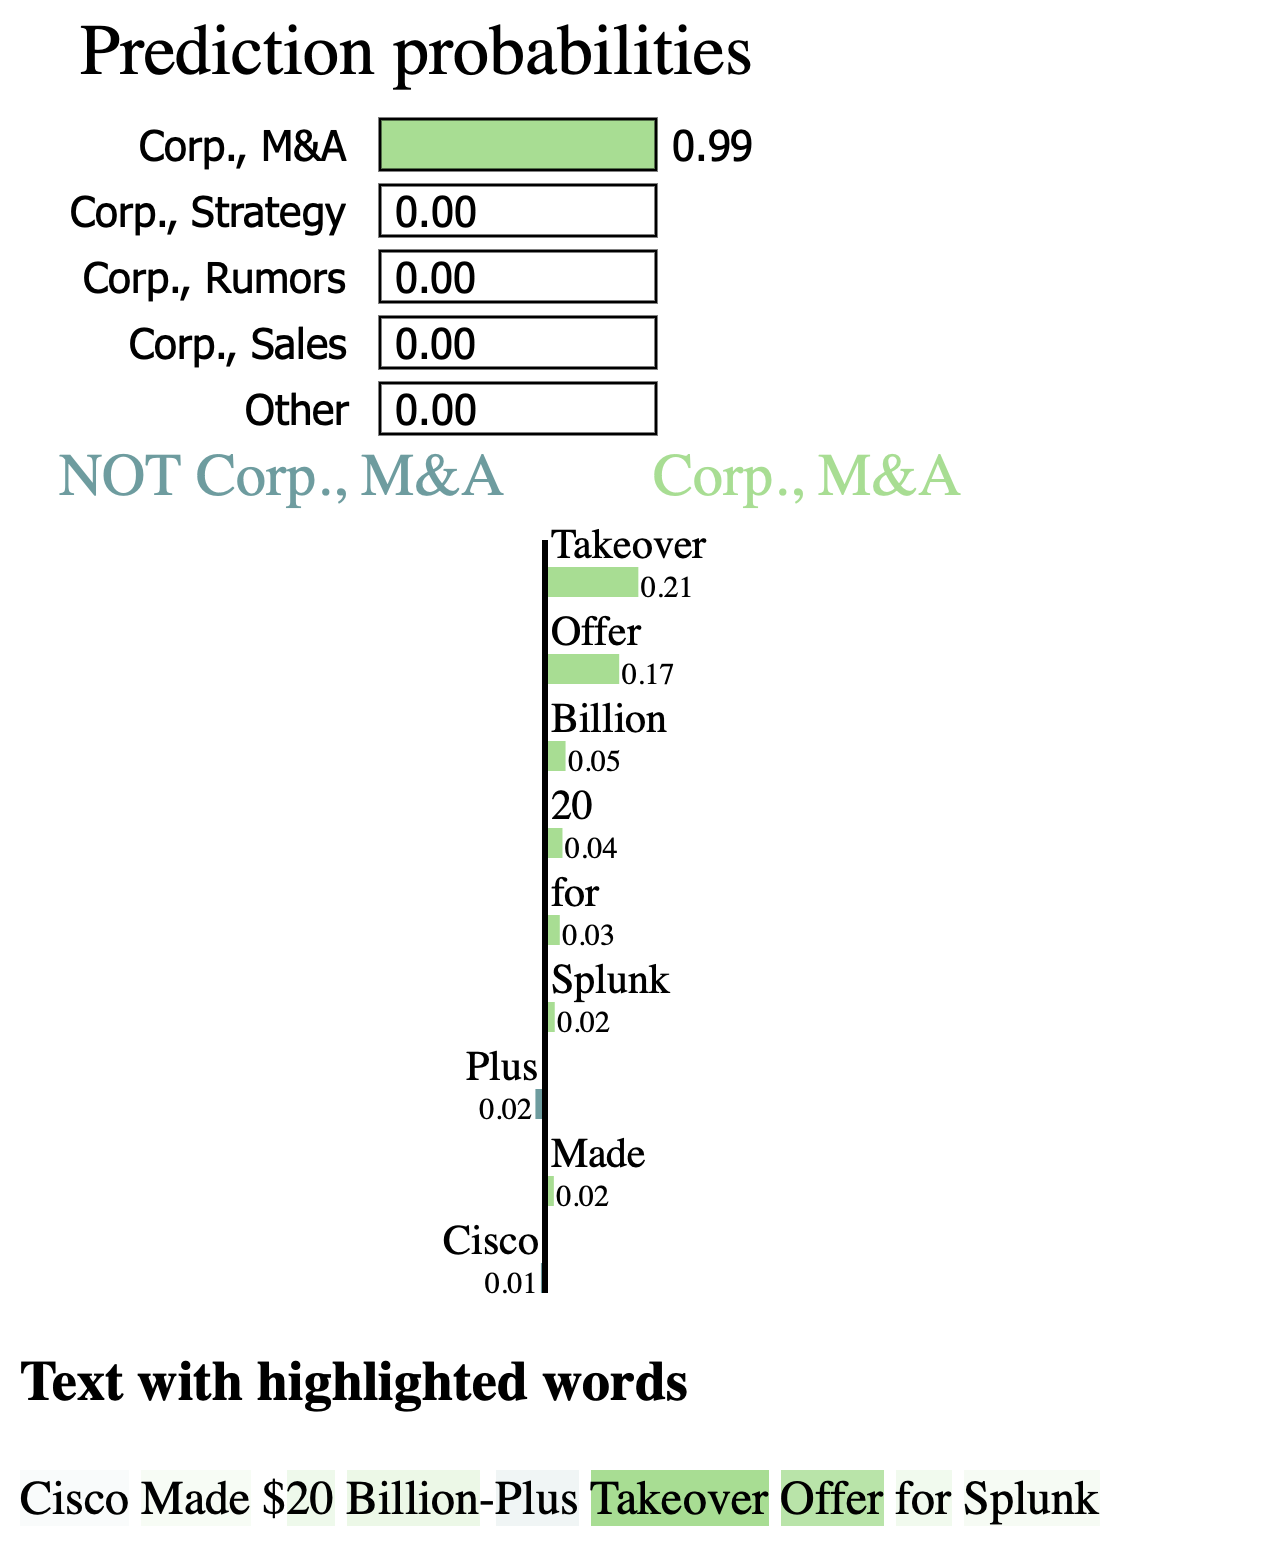
\includegraphics[width=.8\linewidth]{images/lime_m&a.png}
        \label{fig:lime1}
    \end{subfigure}%
    \begin{subfigure}{.5\textwidth}
        \centering
        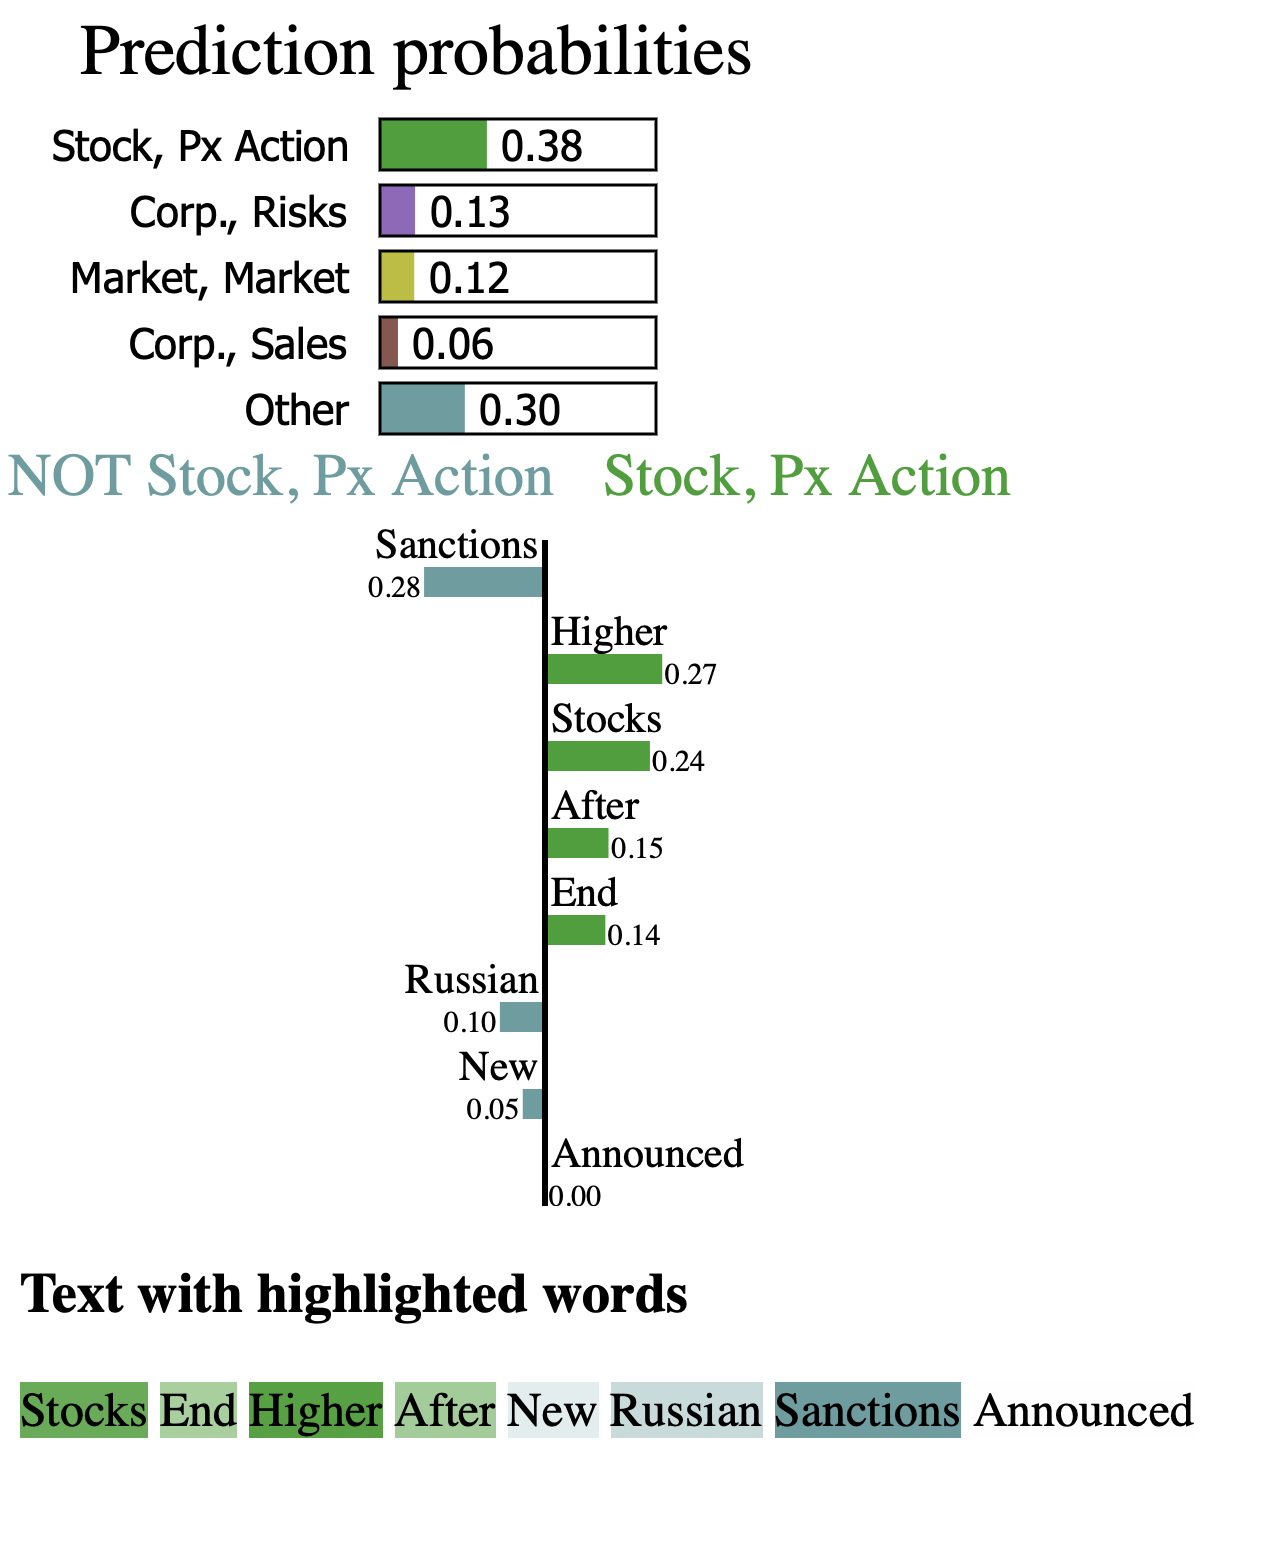
\includegraphics[width=.8\linewidth]{images/lime_price_action_2.png}
        \label{fig:lime3}
    \end{subfigure}
    \caption{LIME Plots of Out-Of-Sample Financial Headlines}
    \label{fig:fig}
\end{figure}

To aid the interpretability of our model, we train multiple locally interpretable model-agnostic explanations (LIME) models~\citep{lime2016} on recent out-of-sample headlines from the Wall Street Journal.

LIME works by perturbing the input sentence, deleting random words.
Using our neural baseline model, LIME then makes aspect class predictions on the perturbed sentence.
These predictions are used to fit a linear regression model.
The resulting LIME model shows the contribution of each word to the neural baseline’s prediction.

Looking at the LIME visuals in figure~\ref{fig:fig}, sometimes a keyword or two can distinguish among aspect classes.
The headline `Cisco Made \$20 Billion-Plus Takeover Offer for Splunk,' shows that the BERT model has learned to associate the phrase `Takeover Offer' with the correct class, `Corporate - M\&A.'
In another example, the phrase `Stocks end higher after' is associated with price movement.



    \section{Conclusions}\label{sec:conclusions}
    \input{conclusions}


    \section{Directions for Future Work}\label{sec:directions-for-future-work}
    % Would like to augment the dataset.
% Would like to try more fine-tuning schemes.


    \section{Acknowledgements}\label{sec:acknowledgements}
    We would like to thank Sean Mason for his suggestions and insightful comments on the code and manuscript.


    \bibliography{fiqa_bib}

%\section{Appendix}

\end{document}